\chapter{Fallstudie}

Es sollen zwei Ampeln nachgebaut werden, die  in einer experimentellen Umgebung die Funktionsweise realer Ampeln zeigen. Eine der Ampeln soll die gelbe LED blinken und die andere soll im normalen Betrieb sein. In diesem Projekt soll der CI/CD Methode von Development bis zum Deployment angewendet werden.

\section{Anforderungen}\label{anforderungen}

In diesem Abschnitt werden die funktionale und nicht-funktionale Anforderungen für die Realisierung des Projekts analysiert.


\subsection{Funktionale Anforderungen}

Die funktionalen Anforderungen beschreiben die gewünschte Funktionalität und das Verhalten des Systems, die in Tabelle\ref{funktionale} aufgelistet sind.


\begin{table}[h!]
	\begin{flushleft}
		{\small 
			\begin{tabular}{|c|c|}
				\hline
				Must-have & 
				\begin{minipage}{5in}
					 \begin{enumerate}
					 	\item Simulierung zwei Verkehrsampeln mithilfe von Raspberry Pi’s und LEDs
					 	\item Automatische Steuerung der LEDs durch GPIO Schnittstelle
					 	\item Entwicklung einer Software für das Blinken der gelben LED
					 	\item Entwicklung einer Software für den Normalbetrieb der Ampel
					 	\item Automatische Software-Test
					 	\item Automatische Bereitstellung (release) der Software
					 	\item Implementierung von \ac{CI/CD} Software-Entwicklungsmethode
					 \end{enumerate}
				\end{minipage} \\
				\hline
				Should-have & 
				\begin{minipage}{5in}
					\begin{enumerate}
						\item Automatische Containerisierung der für das Ampelsystem entwickelten Software mithilfe von Docker
						\item Automatische Veröffentlichung von containerisierten Software auf Docker Hub
						\item Orchestrierung der Docker-Containers mithilfe von Kubernetes
					\end{enumerate}
				\end{minipage} \\
				\hline
				Could-have & 
				\begin{minipage}{5in}
					\begin{enumerate}
						\item Automatische Übertragung (deploy) der Software an das Endgerät
					\end{enumerate}
				\end{minipage} \\
			\hline
			\end{tabular}	
		}
	\end{flushleft}
	\caption{Funktionale Anforderungen}\label{funktionale}
\end{table}



\subsection{Nicht-Funktionale Anforderungen}

Nicht-funktionale Anforderungen beschreiben die Qualität der oben genannten Funktionen, die erreicht werden müssen. Daher haben sie einen erheblichen Einfluss auf Ressourcenverbrauch, Entwicklung und Wartung. Darüber hinaus tragen diese Anforderungen dazu bei, die Akzeptanz des Systems zu verbessern. Einige dieser Anforderungen werden im Folgenden aufgelistet und erörtert.

\begin{itemize}
	\item \textbf{Zuverlässig:} Zuverlässigkeit stellt die Grundvoraussetzung für die Akzeptanz des Systems dar. Das korrekte Verhalten und der Übergang in einen sicheren Zustand im Fehlerfall muss immer gewährleistet sein. Falls die Übertragung der Software in einem inkorrekten Zustand endet, müssen Entwickler in der Lage sein, das System in den korrekten Zustand wiederherzustellen.
	\item \textbf{Skalierbar:} Das Projekt soll skalierbar sein. Wenn man eine neue Ampel nachbauen möchte, sollte es einfach und nicht kompliziert sein.
	\item \textbf{Fehlertoleranz:} Im Falle eines Fehlers sollte die Pipeline die weitere Ausführung anderer Schritte stoppen, wodurch Fehler vermieden werden, die aufgrund einer nachfolgenden Ausführung auftreten können.
	\item \textbf{Robust:} Der Pull-Request soll nicht gemergt werden, bevor die Fehlerfreiheit des Programms durch bestehenden Unit-Test bestätigt wird.
	\item \textbf{Zeiteffizient:} Der gesamte Prozess, von der Entwicklung bis zur Auslieferung, muss in kurzer Zeit und ohne Unterbrechung erfolgen.
	\item \textbf{Echtzeitüberwachung:} Während der Übertragung des Software-Updates soll dieses in Echtzeit überwacht werden.
	
\end{itemize}





\section{Konzept}


\subsection{Geeignete Software-Update-Strategie der Ampelanlage}

Heutzutage sind mehr Geräte mit dem Internet verbunden als je zuvor, was bedeutet, dass Software-Updates über das Internet und nicht über eine traditionelle Schnittstelle bereitgestellt werden müssen. Das spart viel Zeit und Geld bei der Wartung der Software und entlastet vor allem den Facharbeitern. Darüber hinaus wird die Fehlersuche im Fehlerfall durch den einfachen Fernzugriff auf das betroffene System erheblich vereinfacht. 
Diese Strategie wird als Softwar Over The Air (SOTA) benannt. Durch diese Strategie wird die Echtzeitüberwachung der Übertragung ermöglicht, was das ganze Software-Update der Ampelanlage übersichtlicher macht. Darüber hinaus wird durch SOTA Flexibilität bei der Software-Update erreicht, was bedeutet, dass jede Softwareversion mit einem einzigen Klick auf das System übertragen werden kann.
Dies macht die Strategie einfach zu handhaben. Neben all diesen Vorteilen hat das System noch einen weiteren Vorteil, nämlich die Anzahl der Updates ist nicht begrenzt und somit nicht zeitabhängig.


\subsection{Software Update-Architektur der Ampelanlage}

Um die oben genannten Vorteile nutzen zu können, ist es notwendig, eine Internet-Schnittstelle zur Außenwelt zu schaffen. In diesem Zusammenhang und aufgrund der im Raspberry Pi integrierten Internetschnittstelle eignet sich der Raspberry Pi für dieses System,  und weil es sich um ein Minicomputer handelt, erfüllt die in diesem Projekt aufgelistete Anforderungen. Die Abbildung \ref{fig:FW-Update-Strategie} zeigt, wie ein Entwickler, über das im Raspberry Pi integrierte Internetschnittstelle ein Update auf der Ampelanlage übertragen kann, nachdem er die Software auf GitLab hochgeladen hat. Die Verteilung der korrekten Software-Version an den entsprechenden Ampelanlage erfolgt über Raspberry Pis, die direkt mit den Ampelanlagen angeschlossen sind.
\newline\newline
Die Software-Update-Architektur in Abbildung\ref{fig:FW-Update-Strategie} zeigt deutlich, dass für die Anforderungen, die im Abschnitt \ref{anforderungen} aufgelistet sind, eine hierarchische Software-Deployment Topologie dafür geeignet ist. 
\newline\newline
Die Architektur von Kubernetes, die im Kapital {\LARGE ??} beschrieben wurde, bietet die Möglichkeit ein hierarchische Firmware-Deployment aufzubauen.


\begin{figure}[bth] 
	\centering
	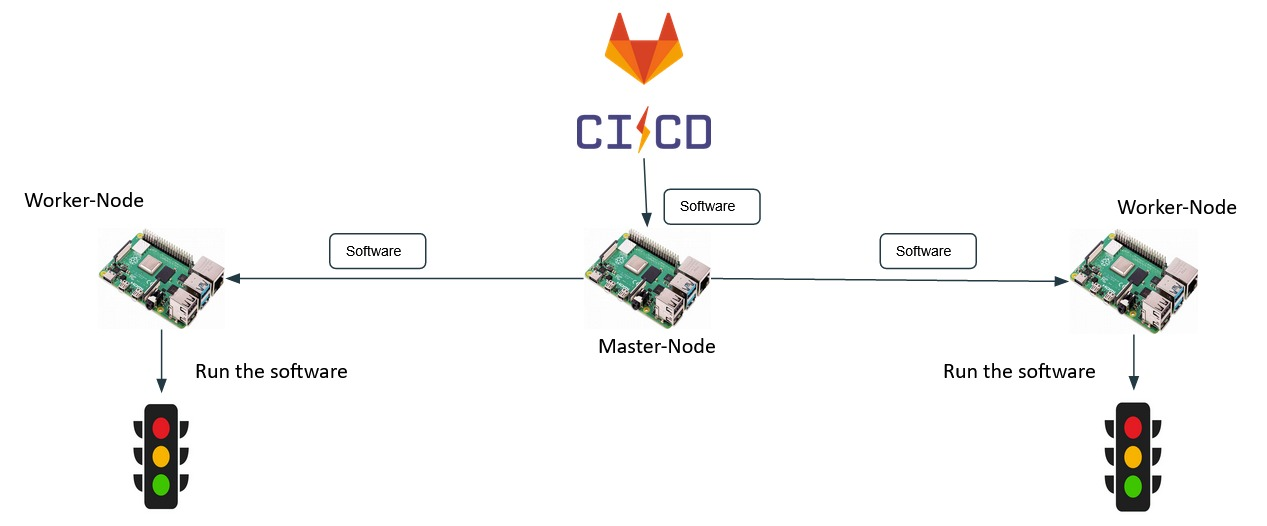
\includegraphics[width=0.7\textwidth]{Graphics/architektur.jpeg}
	\caption{Übersicht der Software Update}
	\label{fig:FW-Update-Strategie}
\end{figure}

\subsection{Auswahl der geeigneten Release-Managementmethode}

Die Unterschiede der Release-Managementmethoden zeigen, dass die CD-Methode es ermöglicht, qualitativ hochwertige Software-Release in kurze Zeit auf einem Endgerät zu übertragen. CD Methode bietet automatisierte Build- , Test- und Deploymentschritte, um vom Menschen verursachte Fehler zu vermeiden, die bei der manuellen Durchführung der Phasen auftreten können. Außerdem können in jeder Phase Probleme auftreten. Abhängigkeiten zwischen den Schritten können eine schnelle Fehlerkorrektur garantieren. Tritt in einer Phase ein Fehler auf, wird die Pipeline unterbrochen und somit weitere Fehler verhindert. Die Software kann nahtlos, sicher, zuverlässig und wiederholt auf dem Endgerät übertragen werden. Darüber hinaus kann der Entwickler den Fortschritt der Phasen beobachten, was hilft, wenn während der Phase ein Fehler auftritt, kann der Entwickler nur ab dieser Phase und nicht von allen Phasen aus iterieren. Bei anderen Release-Managementmethoden benötigen Produkthersteller Releasemanager, um Entscheidungen darüber zu treffen, wann Releases erstellt werden, wie einzelne Schritte ausgeführt werden und wann Software ausgeliefert werden soll. Die Methode CD ermöglicht es dem Release Manager, sich mehr auf die operative Seite zu konzentrieren, wie beispielsweise die Erstellung eines automatisierten Prozesses und Workflows zur sicheren Migration von Code in das Endprodukt, anstatt sich auf die Planungs-, Entwicklungs- und Testphasen zu konzentrieren.



\subsection{Auswahl der geeigneten Release-Strategie}

Die Wahl einer geeigneten Release-Strategie hängt vom Hersteller des Produkts und dem Produkt selbst ab. Bei modernen medizinischen Geräten, Fahrzeuge und IoT Geräte sind Fehlerbehebung und neue Funktionen für einen besseren Service für die Kunden unerlässlich. Daher wird in dieser Fallstudie eine flexible Release-Strategie bevorzugt. Die Schritte im Release-Management-Prozess bleiben generisch, sodass der Wechsel zu anderen Release-Strategien einfach sein kann. Eine flexible Release-Strategie sieht laut Dr.-Ing. Kühn in der Regel die Planung von Änderungen an einem bestimmten Produkt vor\cite{doktor-thesis}.





\section{Entwicklungsvorgang}



\section{Implementierung}


\subsection{Aufbau der experimentellen Umgebung}

Zur Ausführung der vorher ausgewählten SOTA-Methode werden ein Server und ein Client benötigt. Der Server kommuniziert mit dem Client über die in das Produkt eingebaute Internetschnittstelle. Dadurch wird das Update übertragen und während der Übertragung Nachrichten ausgetauscht. Für diese Aktualisierungsmethode ist eine Testumgebung konfiguriert. Die Umgebung umfasst ein Server-zu-Client-Kommunikationssystem. Als Server und Clients werden die Raspberry Pis  zunutze genommen. Ampelanlagen sind mit den Raspberry Pis, die als Client vorgesehen sind, verbunden. In diesem Projekt werden die reale Ampelanlage durch LEDs und Breadboard simuliert, um die serielle Kommunikation zu verwirklichen.
\newline\newline
Außerdem wird die Kubernetes-Cluster konfiguriert, der Master-Node wird auf einem Raspberry pi installiert und die Worker-Nodes sind in dieser Architektur die Raspberry Pis, die jeweils mit einer Ampelanlage verbunden sind. Die installierte Worker-Nodes sollen mit dem Master-Node registriert werden. Um Kubernetes-Anwendungen einfach nutzen und verwalten zu können, wird auch Helm-Tool auf den Master-Node heruntergeladen.

\subsection{Implementierung des Release-Management-Prozesses}

Der Release-Management-Prozess enthält alle notwendigen Schritte, bis die Software auf das Endprodukt verteilt wird. Dies sind die Entwicklung-,Build-,Test- und Deployment-Phase. Sobald der Entwicklungsprozess abgeschlossen ist, erfolgt die automatischen weiteren Phasen wie Build-, Release- und Deployment-Phase. Das Update kann sowohl für alle angeschlossenen Ampelanlagen als auch für verschiedene Ampelanlagen durchgeführt werden. 
\newline\newline
Im Laufe dieses Kapitels wird den ausgewählten Entwicklungsprozessentwurf umgesetzt und wird darauf eingegangen, wie es in der Realität ein Release erstellt wird.
In der Buildphase wird die benötigte Dateien und deren Abhängigkeiten übersetzt und das Ergebnis zur Verfügung gestellt. Diese Phase ist für den gesamten Entwurf und die Implementierung der Architektur erforderlich. Nach der Build- und Release-Phase erfolgt die Deployment-Phase. In dieser Phase wird die Übertragung der Software bis zum Ampelanlage geschehen. Die Ausführung der Phasen erfolgt so weit wie möglich automatisiert und falls während der Ausführung Fehler auftreten, wird die Pipeline unterbrochen, wodurch die Fortsetzung der anderen Phasen verhindert wird.

\subsubsection{Umsetzung der Continues Integration und Continues Delivery Methode}

Nun nach der Entwicklungsphase kommt die CD-Phase zustande. Nach dem Start der CD-Pipeline beginnt die kontinuierliche Deployment-Phase an. Zu CD gehört die Build-,Release- und die Deployment-Phase. Um Continues Integration und Continues Delivery mit GitLab nutzen zu können, wird einen GitLab Runner benötigt. GitLab Runner ist eine Build-Instanz, die verwendet wird, um Aufgaben auf mehreren Computern auszuführen und die Ergebnisse durch „artifacts“ an GitLab zu übertragen.
\newline\newline
In diesem Projekt wird der Gitlab Runner auf dem Master-Node konfiguriert und mit einem Executer vorgesehen, der die vordefinierten Aufgaben in Gitlab aus-
führt. Sobald der Runner registriert ist, initiiert das Runner Tag die Kommunikation zwischen der Gitlab-Plattform und dem Master-Node, auf dem der Runner installiert ist. Die möglichen Executors sind beispielsweise SSH, Shell, Docker, Kubernetes und einige andere. In diesem Projekt wird Kubernetes-Executer benutzt.
\newline\newline
Im
Folgenden werden die einzelnen Phasendurchführungen erklärt.
\subsubsection*{Build-Phase}

Nun wenn die Pipeline gestartet wird, beginnt die Phasendurchführung der CD. Die erste Phase ist die Build-Phase, da in diesem Projekt Programmiersprache Pythen verwendet wird, wird diese Phase nicht in der Pipeline-Phasen hinzugefügt.

\subsubsection*{Test-Phase}

Nachdem der Prozess Merge von DevelopBranch mit  MasterBranch gestartet wird, folgt die \ac{CI/CD}-Testphase. Für die Testphase wird die Master-Node verwendet. In diesem Projekt wird UniTest für den RaspberryPi GPIO ausgeführt. Der Erfolg des Merge-Prozess hängt von den Ergebnissen von UniTest ab. Wenn der Test nicht erfolgreich abgeschlossen werden kann, wird auch der Merge-Prozess abgebrochen, um eine weitere Ausführung der \ac{CI/CD}-Phase zu verhindern.

\subsubsection*{Publish and Release Phase}

Nach erfolgreichem Merge-Prozess kann die weiter \ac{CI/CD}-Phase fortgesetzt werden. Nach der Vergabe des Release-Tags wird die Pipline gestartet und die zweite \ac{CI/CD}-Phase dieses Projektes ist die \glqq Publish and Release Phase\grqq. In dieser Phase wird die entwickelte Software als Docker-Image gekapselt, auf die Dockerhub-Plattform hochgeladen und zur Übertragung und/oder Installation bereitgestellt. Für die Ausführung dieser Phase wird erneuert der Runner der Master-Node benötigt. Durch das Hochladen des Images wird einen neuen Release erstellt. Außerdem wird ein gewohnliche Release auf dem GitLab-Plattform erstellt. Die Abbildung 7.4 veranschaulicht die Release-Phase anhand eines Sequenzdiagramms.
